\documentclass{article}
\usepackage[margin=0.5in,vmargin=0.5in]{geometry}
\usepackage{tikz}
\usepackage{graphicx}

%% neural network parameters
\newcommand\widthCirc{.5} % size of all circles
\newcommand\otdis{8} % distance between layers
\newcommand\nodeSep{2} % node seperation along y axis
\newcommand\inputNodes{5} % input node count
\newcommand\hiddenNodes{1} % hidden node count
\newcommand\outputNodes{0} % output node count
\newcommand\inputSRow{0} % vertical off-set of input layer
\newcommand\hiddenSRow{3} % vertical off-set of hidden layer
\newcommand\outputSRow{1} % vertical off-set of output layer

\newcommand\twohiddenNodes{0} % second hidden layer node count
\newcommand\twohiddenSRow{2} % vertical off-set of second hidden layer


\begin{document}

\begin{centering}

  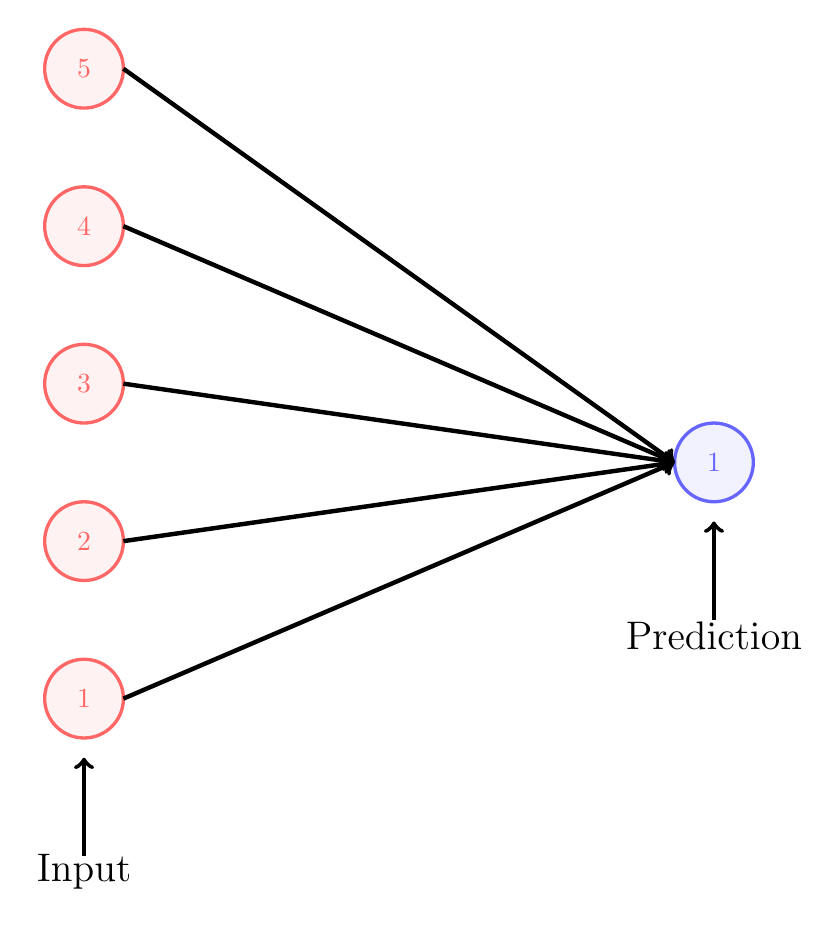
\begin{tikzpicture}
    \foreach \Rnumber in {1,...,\inputNodes}{
      \filldraw[color=red!60, fill=red!5, very thick](0,\inputSRow+\nodeSep*\Rnumber) circle (\widthCirc) node {$\Rnumber$};
    }
    
    \foreach \Rnumber in {1,...,\hiddenNodes}{
      \filldraw[color=blue!60, fill=blue!5, very thick](\otdis,\hiddenSRow+\nodeSep*\Rnumber) circle (\widthCirc) node {$\Rnumber$};
    }
    
    %% add arrows for logit
    \node (A) at (0,\inputSRow-.2) {{\Large{Input}}};
    \draw[ultra thick, ->] (0,\inputSRow) -- (0,\inputSRow+\nodeSep-.75) node {};

    %% add arrows for logit
    \node (B) at (\otdis,\hiddenSRow-.2) {{\Large{Prediction}}};
    \draw[ultra thick, ->] (\otdis,\hiddenSRow) -- (\otdis,\hiddenSRow+\nodeSep-.75) node {};

    \foreach \Rnumber in {1,...,\inputNodes}{
      \foreach \Cnumber in {1,...,\hiddenNodes}{
        \draw[ultra thick, ->] (0+\widthCirc,\inputSRow+\nodeSep*\Rnumber) -- (\otdis-\widthCirc,\hiddenSRow+\nodeSep*\Cnumber) node {};
      }
    }


  \end{tikzpicture}
\end{centering}

\end{document}
